\section{Study Design}\label{sec-content}
\noindent
The overall study consists of three parts. In each part, we ask participants to implement specific parts of the architecture using capabilities via external libraries or via module systems in languages. Each part was designed to primarily test one of the facets of the overall goal (usability, extensibility, and security); however, all facets were considered in the analysis of each part.

Each study part was divided into three steps for participants - designing the initial architecture, finding vulnerabilities, and the post-study survey.\footnote{Code templates for the studies are available at \url{https://github.com/abhaasgoyal/module-systems/tree/plateau-2024}} 

\subsection{Logger Editor} \label{sec:loggerEditor}
\begin{figure}[htbp]
\centering
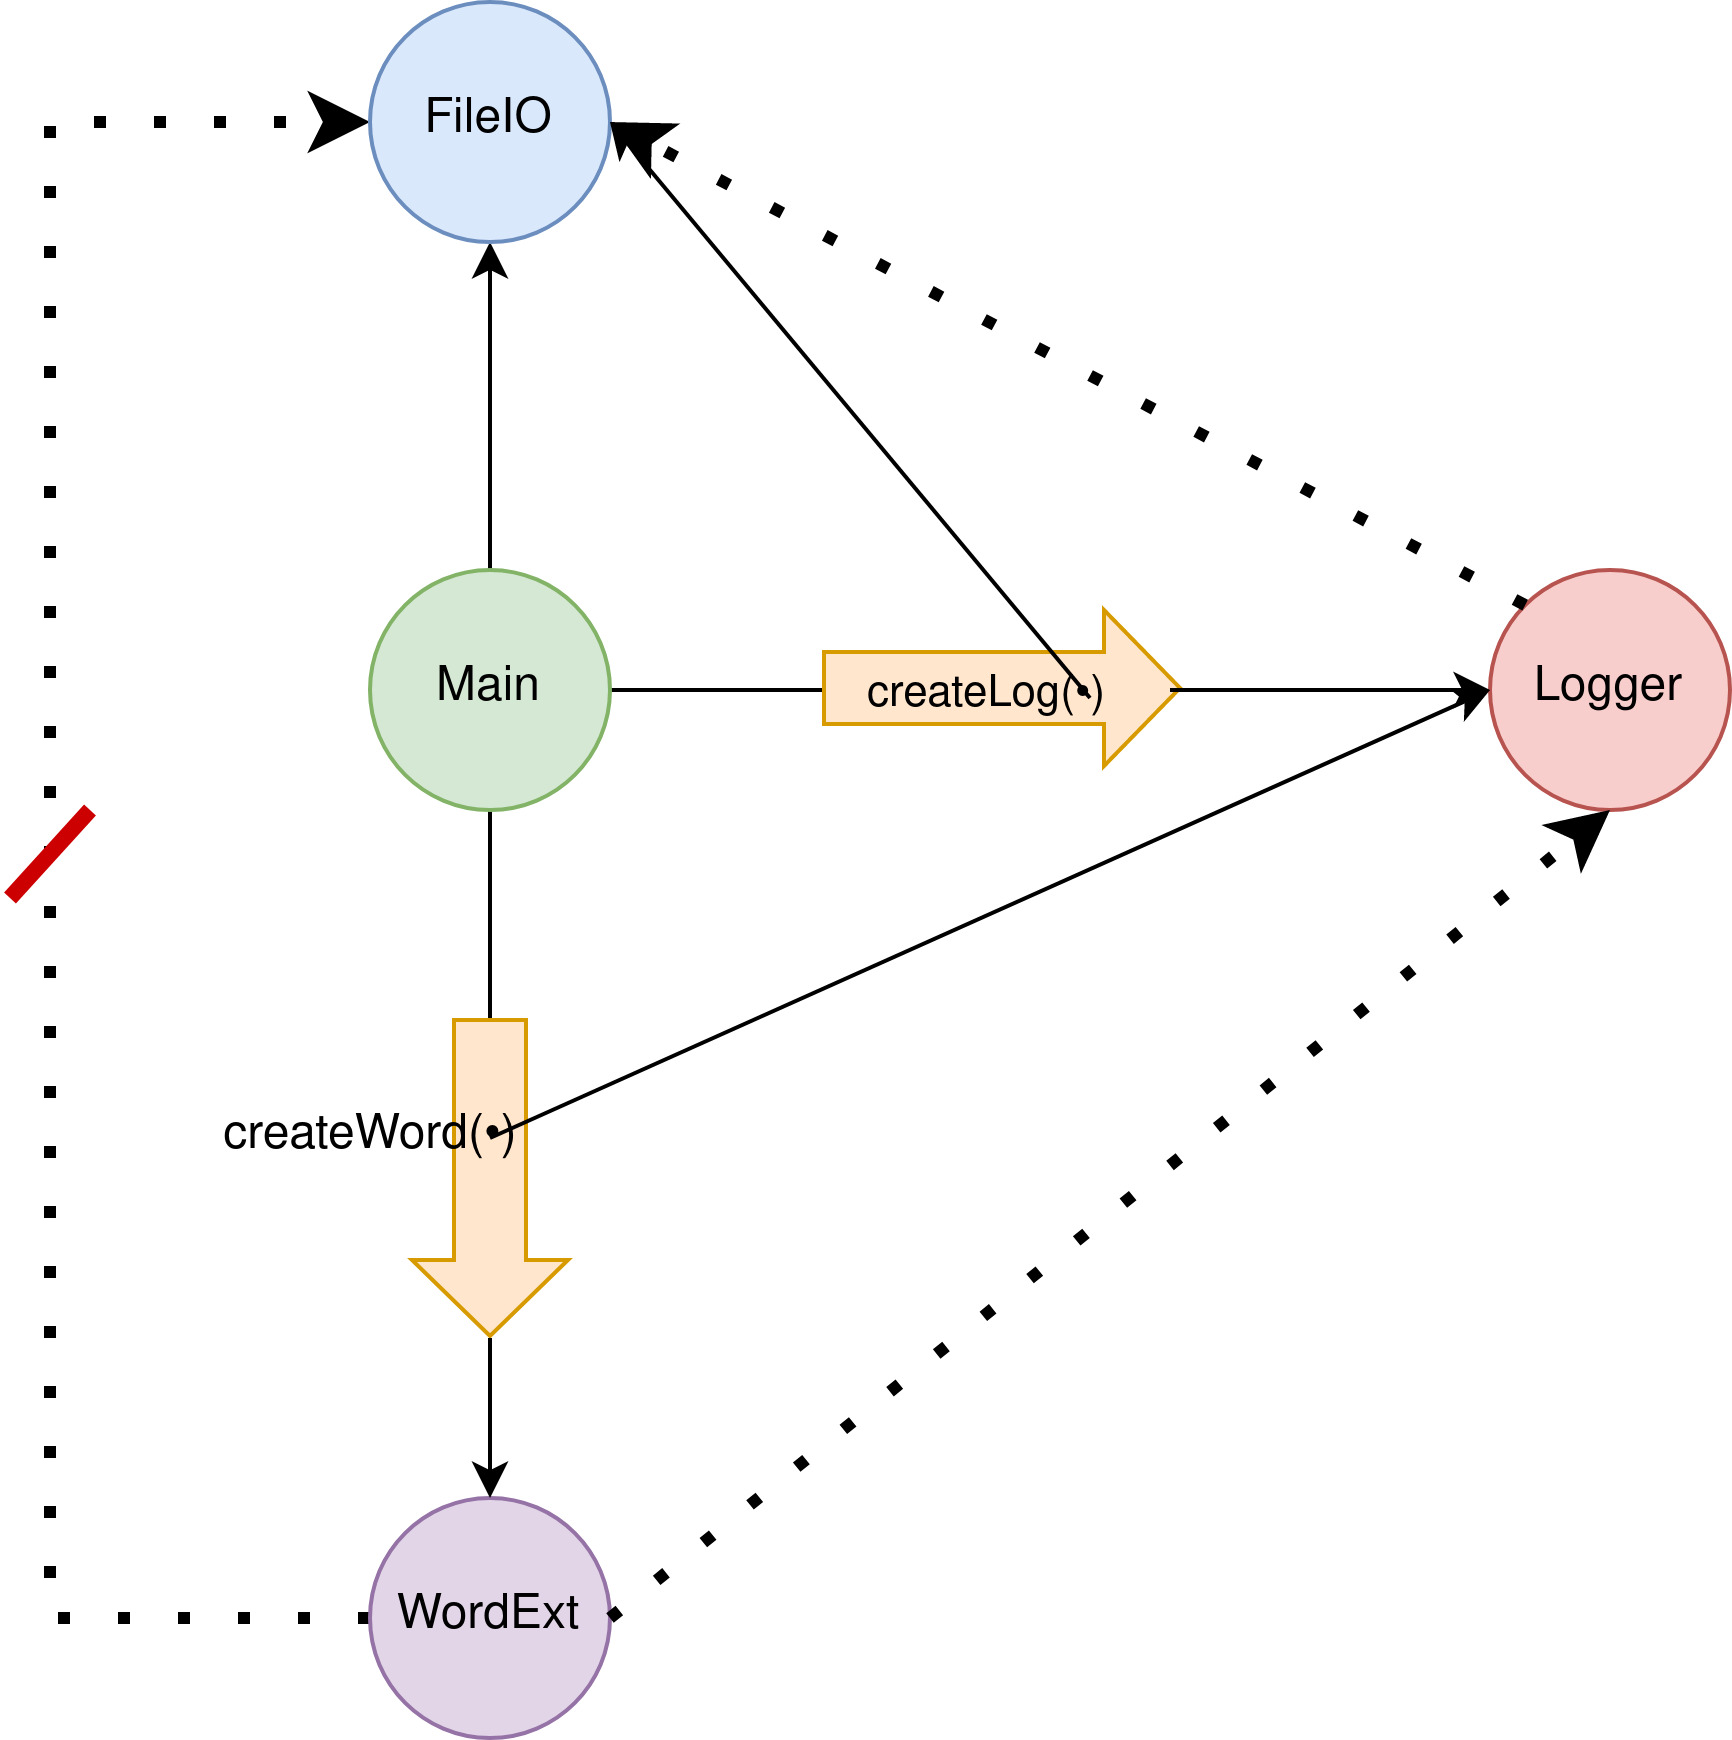
\includegraphics[width=2.2in]{figures/Ambient_logger.jpg}
\caption{Logger Editor}
\label{loggerEditor}
\end{figure}
\noindent
\textbf{Purpose} To assess the security of participant code, ensuring that authority is non-transitive.

% https://drops.dagstuhl.de/opus/volltexte/2017/7270/pdf/LIPIcs-ECOOP-2017-20.pdf
\noindent
\textbf{Background} In figure \ref{loggerEditor}, the \texttt{Main} application has a \texttt{Logger} module that it can trust. The logger module has access to \texttt{FileIO}, providing it the authority to read/write to files. However, there also exists an extension named \texttt{wordCloud} module, which needs to utilize the \texttt{Logger} library to read/write to a place that only \texttt{Logger} can allow. Here, \texttt{Main} passes \texttt{Logger} when creating \texttt{wordCloud}. The goal of the user is to design \texttt{Logger} in such a way that \texttt{WordExt} does not have access to the underlying module \texttt{fileIO} and, in the process, escalate its privilege.

% \noindent
% \textbf{Additional Specifications}
% The following requirements need to be satisfied when designing the logger architecture for specific languages:
% \begin{itemize}
%     \item The name of the log file should be \texttt{log.txt}
%     \item The directory containing the file would depend on the language as follows:
%     \begin{itemize}
%         \item \textbf{Rust} Stored in the env variable \texttt{\$DATA\_DIR} (since Rust's capability library provides inbuilt support for writing directly to that folder)
%         \item \textbf{Wyvern} Stored within the same folder as the program
%     \end{itemize}
% \end{itemize}
\subsubsection{Instructions}
\noindent
\textbf{Rust Implementation}
The implementation in Rust was based on the \texttt{cap-std} module \cite{rustCap}. The implementation should contain the functionalities for the following (note that one can change the function names in the Extension depending on how the Logger is structured): 

\begin{itemize}
    \item \mintinline{Rust}{create_logger(logFile: String)} - A constructor which returns a new logger object with the name logFile
    \item \mintinline{rust}{logFile.append_to_log(entry : String)} - Append a new entry to the logFile
\end{itemize}


Given a possibly malicious \mintinline{Rust}{extension.rs}, design the corresponding Logger module with capability library in Rust.

\noindent
\textbf{Wyvern Implementation} The extension library is \texttt{wordCloud}, and the users need to design the logger library from scratch with the \texttt{appendLog} function. Since capabilities are hierarchical here, the users were given a more open-ended specification of the parameters of the logger library; the solution is that the underlying \texttt{fileIO} system resource is passed exclusively to the logger from Main.

There was no developer-friendly documentation available for Wyvern's standard I/O library, so we provided the implementation, hoping that it will act as self-documenting code. The required method definitions for \texttt{fileIO} are provided in listing \ref{code:fileIOwyv}.

\noindent
\textbf{Trying to Break security} Upon completing the corresponding functions, users were asked to find a way to bypass the restriction of accessing \texttt{fileIO} in the corresponding programs, while only modifying \texttt{Extension.rs} (for Rust) and \texttt{wordCloud} module (for Wyvern).

\subsection{Network Pool}\label{sec:networkPool}

\begin{figure}[htbp]
\centering
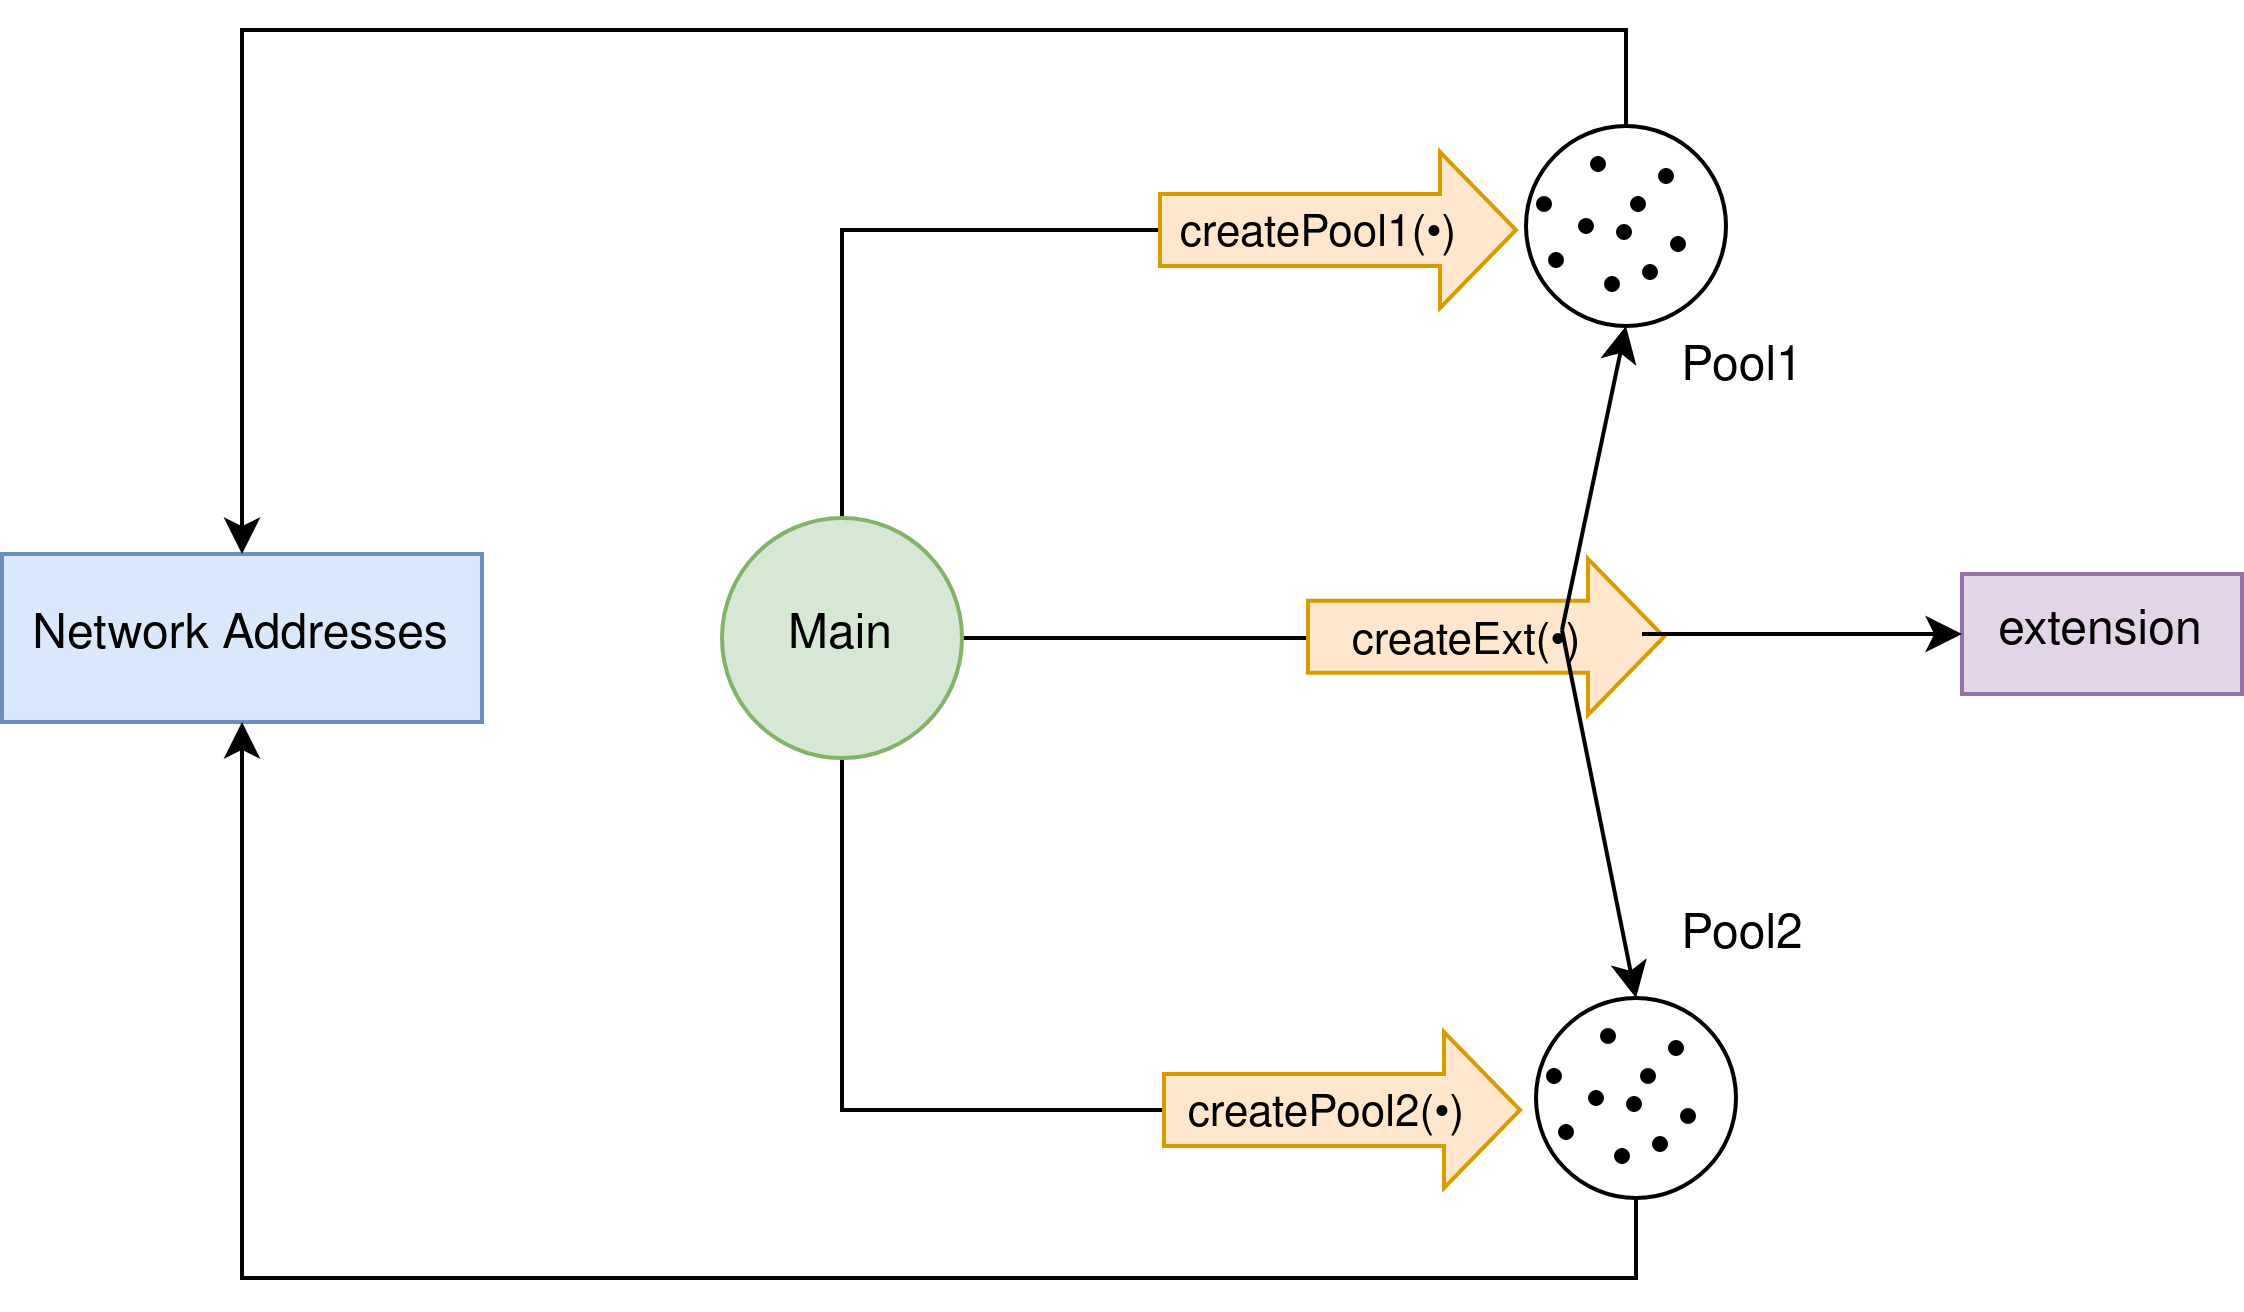
\includegraphics[width=2.8in]{figures/network.jpg}
\caption{Network Pool (A dotted circle is the capability to connect to a specific device)}
\label{fig:network}
\end{figure}

\noindent
\textbf{Purpose} To assess the ease of developing appropriate implementations from the specification. A high degree of freedom should be provided in how to design programs.

\noindent
\textbf{Goal} Firewalls are essential to control incoming and outgoing network traffic. The user has to implement a basic firewall by making two kinds of network pools that allow an untrusted extension to use the network in limited ways. The extension promises to only connect to the website \texttt{example.com}. The architecture can be represented with figure \ref{fig:network}. There are two types of pools used in the Extension. The pools should limit the extension to the following authorities, respectively:

\begin{itemize}
    \item \textbf{TCP-Port} Only allow connections to an IP address of \texttt{93.184.216.14} using a TCP port (0-65535). For Wyvern, it can be assumed that the IP address is a string of fixed length i.e.\ it has a length of 15. For example, \texttt{192.68.1.1} is represented as \texttt{192.068.001.001}
    \item \textbf{Net-Port} Only allow connections to a small range of IP addresses (but with any port allowed). The last 8 bits of the IP addresses should be in the range \texttt{93.184.216.<0-255>}
\end{itemize}

\subsubsection{Instructions}
\noindent
\textbf{Rust Implementation} Within \texttt{pool\_auth.rs}, create the respective network pools by looking at the necessary documentation. Then, call in the Extension by passing in the Pools with the required IP address and HTTP port in both cases as the input. In this case, the necessary documentation was regarding Network Pools implementation  in capability standard library of Rust \cite{libcaprustpool}.
 

\noindent
\textbf{Wyvern Implementation} The \texttt{makePool} module should have 4 input parameters - \texttt{startIp}, \texttt{endIp}, \texttt{startPort}, and \texttt{endPort}.
Then, come up with an abstraction of functions for Net-Port and TCP-Port, which call \texttt{makePool}. This should be within the main function.
Finally, the function \texttt{connect(addr, port)} should consist of a guard which checks whether the \texttt{addr} and \texttt{port} are within the acceptable range, and connects if the check succeeds.

\noindent
\textbf{Trying to Break security} This exercise was similar to the Logger-Editor design, but now considering multiple capabilities that are passed to the Extension. Upon completing the corresponding functions, try to break the security of the filesystem in the corresponding programs by modifying only \texttt{Extension.rs} (for Rust) and the \texttt{cloud} module (for Wyvern).

\subsection{Simple Money} \label{sec:simpleMoney}
\noindent
Note: The design was motivated by the simple money example \cite{millerFinancial}.

\begin{figure}[htbp]
\centering
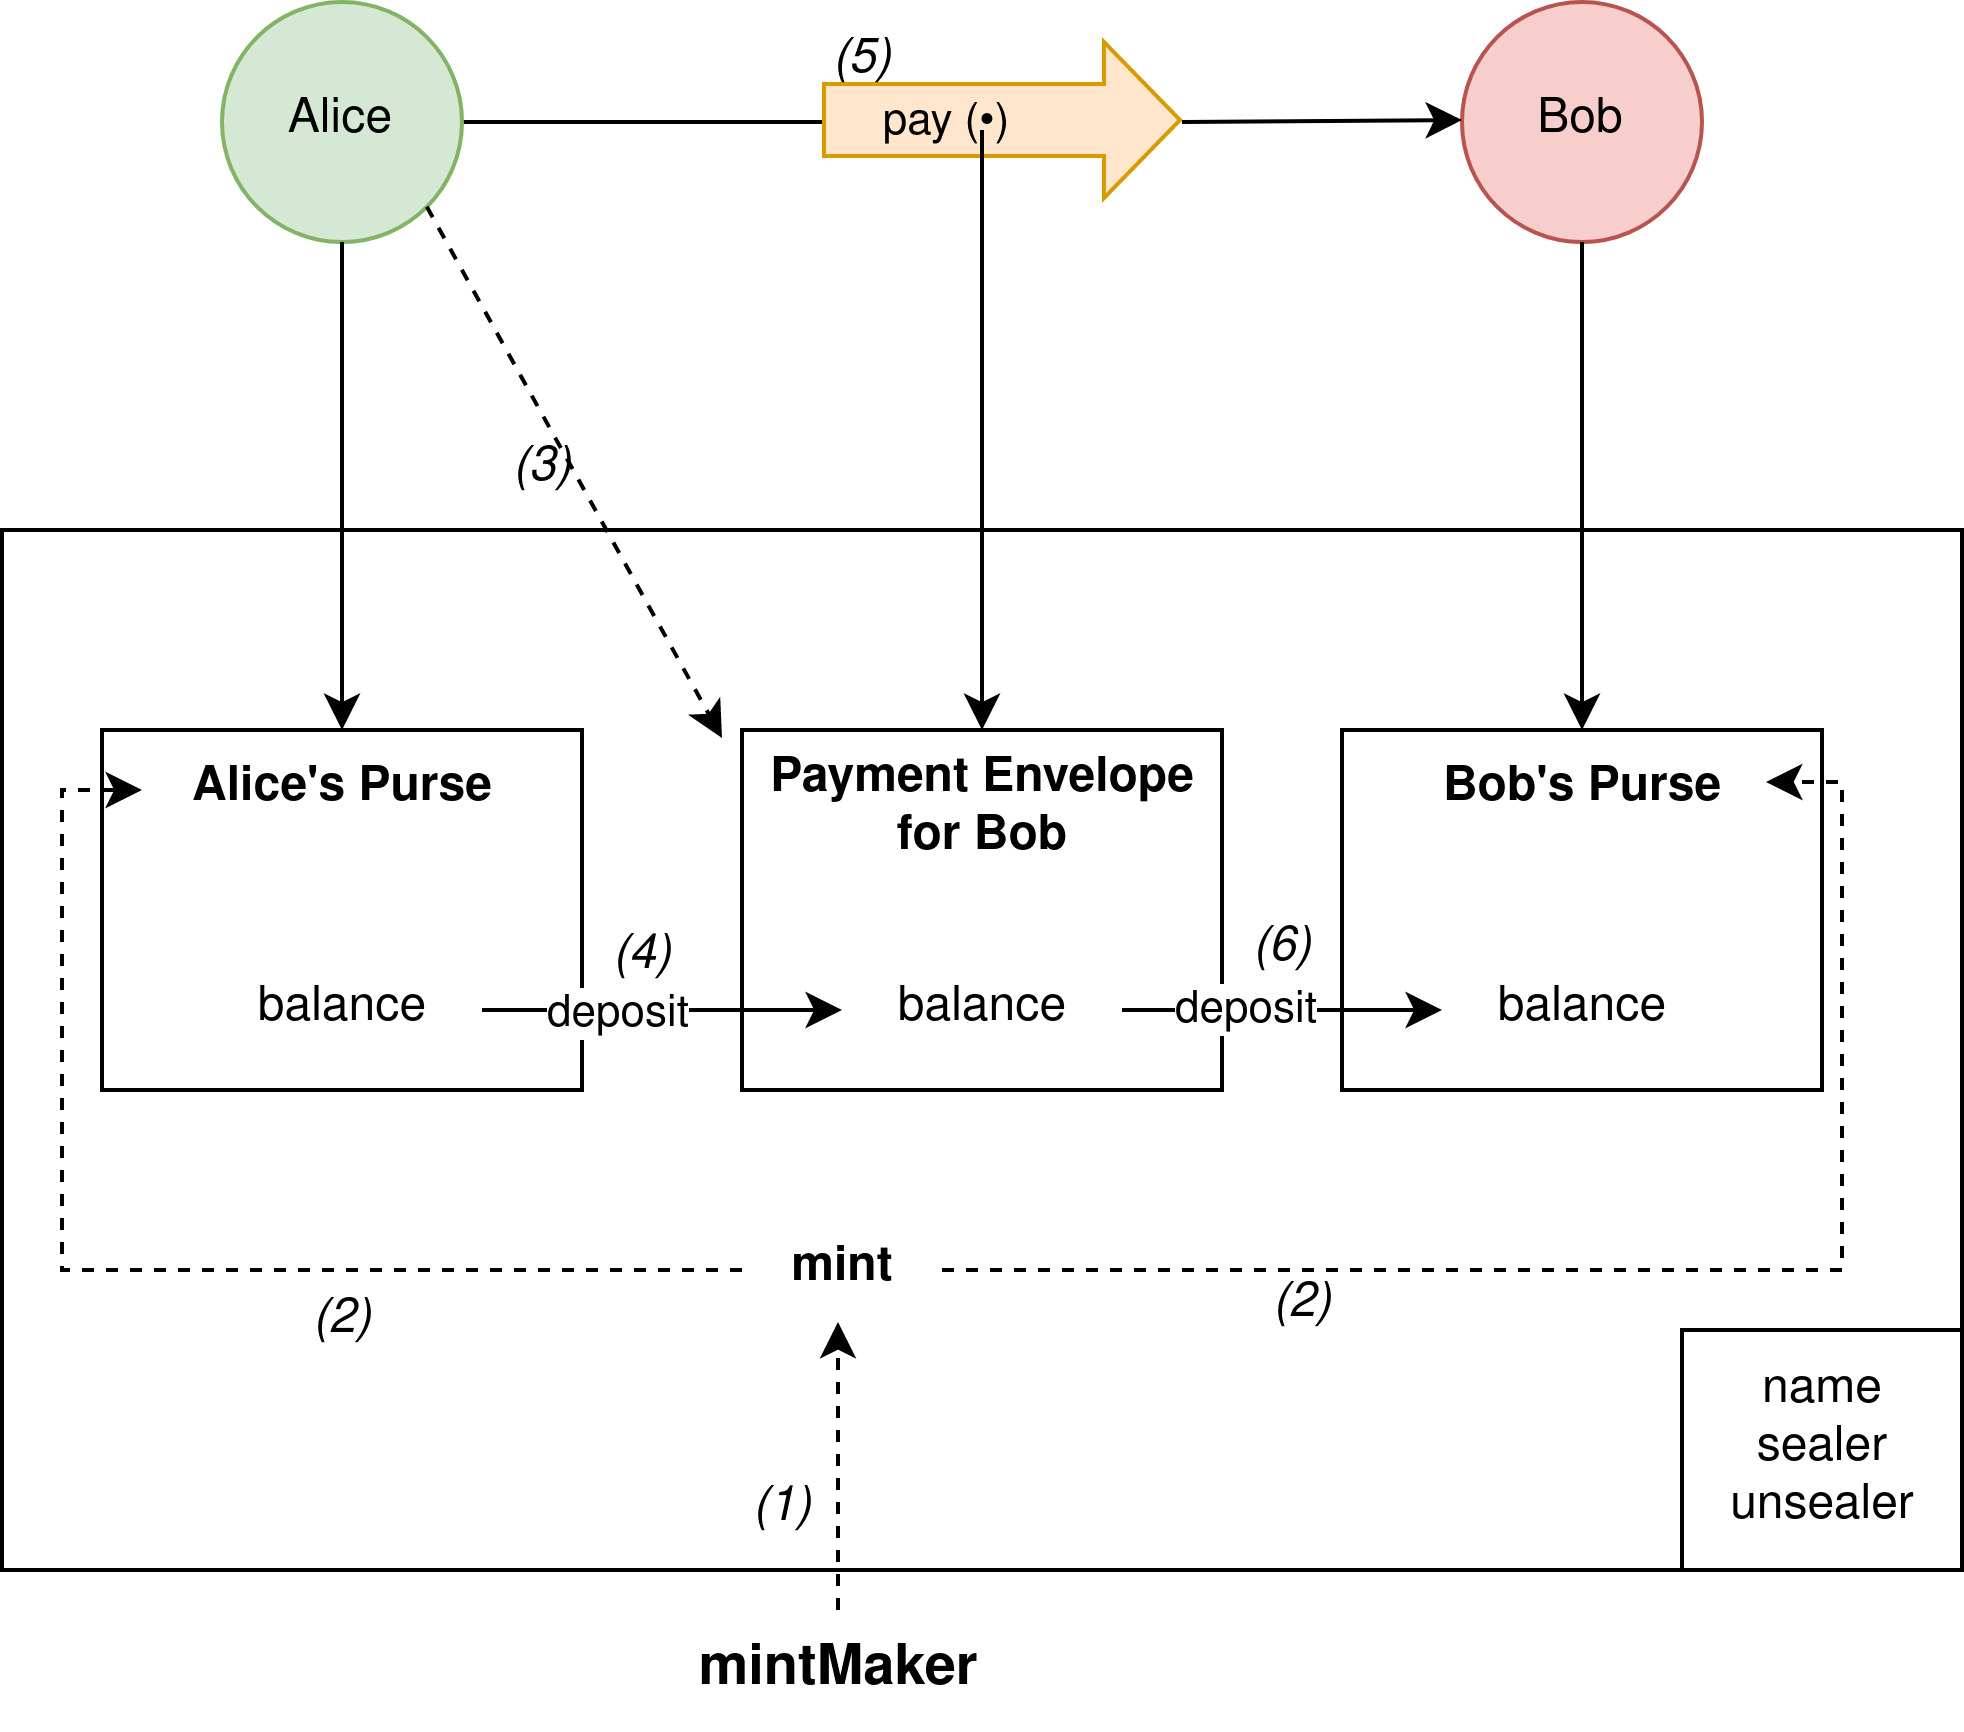
\includegraphics[width=2.6in]{figures/simpleMoney.jpg}
\caption{\label{fig:simpleMoney} Simple Money}
\end{figure}

\noindent
\textbf{Goal} Extensibility of adding code to existing codebases.

\noindent
\textbf{Background} Given a money minter and two purses A and B, design a transaction where user A can securely send money to user B, using the capability pattern of sealer-unsealer. 

\noindent
\textbf{Architecture}
The architecture (figure \ref{fig:simpleMoney}) consisted of the main entity \texttt{mintMaker}, making the \texttt{Mint} Object, representing a new currency. It has a fixed amount of total balance. It employs the Factory Pattern to further create two \texttt{Purse} objects, Alice and Bob, which it can initialize with a certain balance. This is implemented in steps (1)-(2). Now, the question is whether Alice can pay some of her money to Bob while conserving the total currency. Some of the goals the architecture needs to achieve \cite{millerFinancial} are:
\begin{itemize}
    \item (T1) Only someone with the mint has the power to change the total balance of that currency
    \item (T2) \texttt{Purse A} cannot change the balance of \texttt{Purse B}
    \item (T3) Balances should always be positive
    \item (T4) If a successful deposit gets reported, Alice should be guaranteed that the deposit was made to the other wallet
\end{itemize}

\subsubsection{Instructions}
\noindent
The participant is given implementations of the Sealer and Unsealer primitives, as well as the Mint object (steps (1)-(2) in the diagram). The user tasks for both languages were to securely transfer money via an intermediate Purse Object with the Sealer-Unsealer pattern. The purse should have the following methods:
\begin{enumerate}
    \item \mintinline{rust}{purse.getBalance(): Int} - Get the current balance in the purse  
    \item \mintinline{rust}{sprout(): Purse} - Create a new empty purse 
    \item \mintinline{rust}{getDecr(): SealedBox[Int -> void]} - Get a sealed version of \texttt{decr}. A hint was provided that should be used to validate (T4) during a \texttt{deposit} to Bob's purse. \texttt{decr} is a function that subtracts the balance in the current Purse
    \item \mintinline{rust}{dst.deposit(amount:Int,src:Purse):void} - Securely transmits money from one wallet to another
    \item \mintinline{rust}{print():void} - (Optional) Print debugging information
\end{enumerate}

The programmer's expected steps are to understand the respective codebase and extend the program's functionality. Instructions were the same for Wyvern and Rust implementation, with slightly different filenames. They were to implement the architecture above and then come up with potential vulnerabilities in their implementation.